\section{Kết quả truy xuất tài liệu}\label{sec:eval-rag}

Gia sư tìm trong kho tài liệu của giáo viên những đoạn để dựa vào khi học sinh hỏi. Mục này đo ba điều: hệ thống có tìm đúng đoạn không, thành phần nào đóng góp nhiều nhất, và cách tìm có ràng buộc theo thứ tự bài học có tránh được việc dạy trước nội dung chưa học không. Kho gồm $221$ đoạn của hai chương Toán, mỗi đoạn gắn với bài của nó. Năm bộ câu hỏi ở Bảng~\ref{tab:eval-sets} có bốn loại câu: về bài đang học, về bài trước, về bài sau mà học sinh chưa học, và Toán ngoài chương hoặc lạc đề. Phép đo dừng ở chỗ đoạn nào được tìm ra, chưa đo chất lượng câu trả lời cuối cùng mà học sinh đọc.

\subsection{Mỗi thành phần đóng góp bao nhiêu}
Hình~\ref{fig:rag-hit3} so sáu cách tìm. Ba cách đầu, gồm tìm theo từ khóa, theo vector và tìm lai, gần như giống nhau: ở Bộ 2 cả ba cho Hit@3 bằng $0{,}40$ và MRR từ $0{,}449$ đến $0{,}460$. Nguyên nhân nằm ở dữ liệu: văn bản của giáo viên ngắn và dùng chung nhiều thuật ngữ giữa các bài (``phần nguyên'', ``hàng'', ``dấu phẩy''), nên đoạn của bài đang học và của bài khác khớp từ khóa và nghĩa gần như nhau. Điều phân biệt hai loại đoạn là cấu trúc, tức học sinh đang ở bài nào. Cấu hình của đồ án, tức tìm lai kèm các bước dựa vào thứ tự bài học, đạt MRR $0{,}954$ ở Bộ 2 và $0{,}935$ ở Bộ 4, so với $0{,}460$ và $0{,}343$ của tìm lai thuần; ở Bộ 2 mức tăng là $0{,}494$ (khoảng tin cậy từ $0{,}306$ đến $0{,}678$), với mười một câu chuyển từ sai sang đúng và không câu nào ngược lại. Cách tìm phẳng, không dùng thông tin bài đang học, đứng giữa với MRR $0{,}839$ và $0{,}742$.

\begin{figure}[H]
\centering
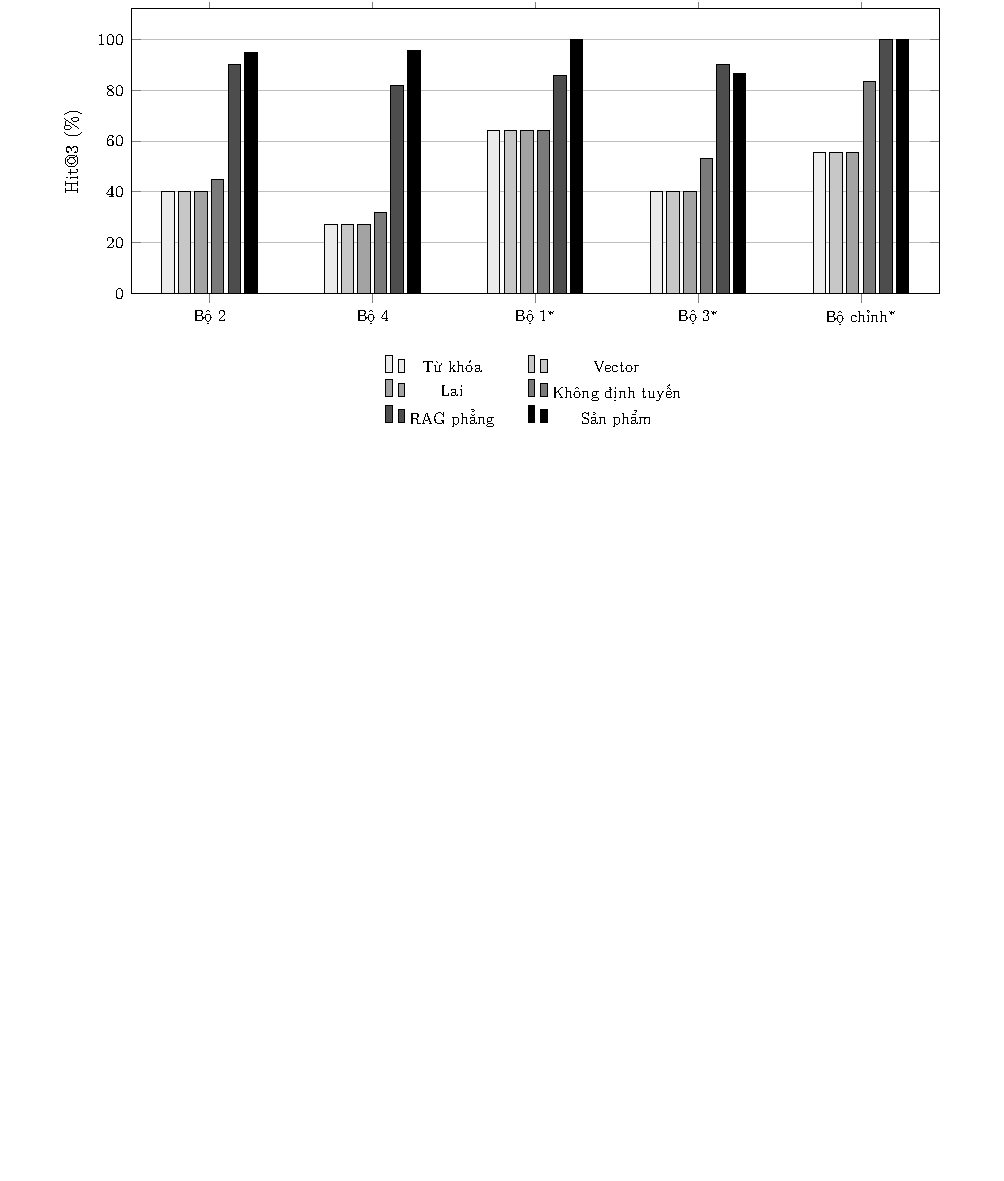
\includegraphics{figures/pdf/fig-rag-hit3.pdf}
\caption{Hit@3 của sáu cách tìm trên năm bộ câu hỏi. Dấu $^{*}$: bộ đã dùng để chỉnh thiết kế (không độc lập).}
\label{fig:rag-hit3}
\end{figure}

Bảng~\ref{tab:rag-components} bỏ riêng từng thành phần khỏi cấu hình của đồ án rồi xem kết quả giảm bao nhiêu. Định tuyến theo chủ đề là thành phần quyết định: bỏ nó làm MRR giảm $0{,}450$ ở Bộ 2 (khoảng tin cậy từ $0{,}263$ đến $0{,}642$, $p=0{,}002$) và $0{,}550$ ở Bộ 4 ($p<0{,}001$). Tìm theo vector đứng thứ hai với mức giảm $0{,}224$ và $0{,}242$ nhưng chưa đủ bằng chứng thống kê ($p=0{,}125$ và $0{,}070$ trên hai bộ nhỏ). Giới hạn theo thứ tự bài đóng góp $0{,}114$ và $0{,}193$. Bỏ tìm theo từ khóa gần như không đổi gì, và hai bước xếp hạng lại cuối không đổi gì ở các bộ này vì định tuyến đã đưa đoạn đúng lên đầu. Dữ liệu vì vậy phù hợp với nhận định rằng tìm theo ngữ nghĩa chỉ phát huy khi đi cùng cấu trúc bài học, nhưng chưa đủ để khẳng định vector có ích độc lập. Về các hệ số của xếp hạng lại ($\kappa_m$ theo loại đoạn, $\gamma$ theo ngữ cảnh), đồ án nâng mọi $\kappa_m$ lên lũy thừa từ $0$ đến $2$ và đổi từng $\gamma$ trong khoảng $[1;2]$: Hit@3 và MRR trên Bộ 2, 3 và 4 không đổi (lệch tối đa $0{,}001$). Kết quả này chưa biện minh các hệ số, vì nhãn coi mọi đoạn của bài là đúng nên đổi loại đoạn không đổi thứ hạng và chỉ có $3$, $9$ và $3$ câu thuộc chế độ dùng hệ số; các hệ số là lựa chọn thiết kế cần một tập đo riêng việc chọn loại đoạn.

% Sinh bởi tools/paper_tex.py từ docs/paper/data; không sửa tay.
\begin{table}[H]
\centering
\caption{Bỏ từng thành phần khỏi cấu hình sản phẩm: thay đổi MRR so cặp theo câu và $p$ của McNemar trên Hit@3. Số âm: thành phần có ích.}\label{tab:rag-components}
\small
\begin{tabular}{lrrrr}
\toprule
 & \multicolumn{2}{c}{Bộ 2} & \multicolumn{2}{c}{Bộ 4} \\
\cmidrule(lr){2-3}\cmidrule(lr){4-5}
Thành phần bị bỏ & $\Delta$MRR & $p$ & $\Delta$MRR & $p$ \\
\midrule
Định tuyến chủ đề & $-0{,}450$ & $0{,}002$ & $-0{,}550$ & $<0{,}001$ \\
Vector (ngữ nghĩa) & $-0{,}224$ & $0{,}125$ & $-0{,}242$ & $0{,}070$ \\
Phạm vi theo đồ thị tri thức & $-0{,}114$ & $1{,}000$ & $-0{,}193$ & $0{,}375$ \\
Từ khóa & $-0{,}001$ & $1{,}000$ & $-0{,}023$ & $1{,}000$ \\
Xếp hạng lại sư phạm & $0{,}000$ & $1{,}000$ & $0{,}000$ & $1{,}000$ \\
Ưu tiên đoạn định nghĩa & $0{,}000$ & $1{,}000$ & $0{,}000$ & $1{,}000$ \\
\bottomrule
\end{tabular}
\end{table}


\subsection{Tác dụng của định tuyến và việc tránh dạy trước}
Phiên bản đầu của cách tìm có giới hạn theo bài làm hỏng câu hỏi về bài trước, vì giới hạn đẩy đoạn của bài đang học lên trước đoạn thật sự trả lời. Định tuyến theo chủ đề sửa điều đó (Bảng~\ref{tab:rag-routing}): Hit@3 tăng từ $0{,}45$ lên $0{,}95$ ở Bộ 2 với mười câu được sửa và không câu nào hỏng ($p=0{,}002$), và từ $0{,}32$ lên $0{,}95$ ở Bộ 4 với mười bốn câu được sửa ($p=0{,}0001$). Chiều tác dụng giống nhau ở ba bộ còn lại; hai bộ nhỏ nhất chưa đủ câu để đạt mức ý nghĩa thông thường.

% Sinh bởi tools/paper_tex.py từ docs/paper/data; không sửa tay.
\begin{table}[H]
\centering
\caption{Tác dụng của định tuyến chủ đề trên Hit@3. Đã sửa: số câu chuyển từ sai sang đúng; hỏng: số câu ngược lại; $p$: kiểm định McNemar chính xác.}\label{tab:rag-routing}
\small
\begin{tabular}{lrrrrrr}
\toprule
Tập & $n$ & Không định tuyến & Có định tuyến & Đã sửa & Hỏng & $p$ \\
\midrule
Bộ 2 & 20 & $0{,}45$ & $0{,}95$ & 10 & 0 & $0{,}002$ \\
Bộ 4 & 22 & $0{,}32$ & $0{,}95$ & 14 & 0 & $<0{,}001$ \\
Bộ 1$^{*}$ & 14 & $0{,}64$ & $1{,}00$ & 5 & 0 & $0{,}062$ \\
Bộ 3$^{*}$ & 30 & $0{,}53$ & $0{,}87$ & 10 & 0 & $0{,}002$ \\
Bộ chỉnh$^{*}$ & 18 & $0{,}83$ & $1{,}00$ & 3 & 0 & $0{,}250$ \\
\bottomrule
\end{tabular}
\end{table}


Điều mà giới hạn theo thứ tự bài mang lại so với cách tìm phẳng không nằm ở Hit@3, vốn cao ở cả hai ($0{,}90$ so với $0{,}95$ ở Bộ 2), mà ở chỗ đoạn nào lọt vào kết quả đầu. Bảng~\ref{tab:rag-flat} đếm số câu mà kết quả đầu có đoạn của bài học sinh chưa học: cách tìm phẳng làm vậy ở $56$ trên $163$ câu ($34\%$), cấu hình của đồ án không làm ở câu nào, và với riêng câu hỏi về bài sau cách tìm phẳng đưa nội dung bài đó vào câu trả lời ở $4$ trên $4$ câu ở Bộ 2. Bảng còn cho thấy cách tìm phẳng vẫn trả lời $7$ trên $39$ câu Toán ngoài chương hoặc lạc đề, so với $2$ trên $39$ của đồ án. Đây là bảo đảm cấu trúc của bất biến không dạy trước (B5), mà xếp hạng theo độ giống một mình không cho được.

% Sinh bởi tools/paper_tex.py từ docs/paper/data; không sửa tay.
\begin{table}[H]
\centering
\caption{Đoạn của bài sau lọt vào kết quả đầu và câu ngoài chương bị trả lời. Cột ``bài sau'': số câu hỏi mà kết quả đầu có đoạn của bài học sinh chưa học; cột ``ngoài chương'': số câu Toán ngoài chương mà hệ vẫn trả lời, trên số câu loại này.}\label{tab:rag-flat}
\small
\begin{tabular}{lrrrrr}
\toprule
 & & \multicolumn{2}{c}{Bài sau lọt vào} & \multicolumn{2}{c}{Ngoài chương bị trả lời} \\
\cmidrule(lr){3-4}\cmidrule(lr){5-6}
Tập & Số câu & RAG phẳng & Sản phẩm & RAG phẳng & Sản phẩm \\
\midrule
Bộ 2 & 30 & 11 & 0 & 1/6 & 0/6 \\
Bộ 4 & 37 & 11 & 0 & 3/11 & 2/11 \\
Bộ 1$^{*}$ & 23 & 9 & 0 & 1/6 & 0/6 \\
Bộ 3$^{*}$ & 43 & 13 & 0 & 1/8 & 0/8 \\
Bộ chỉnh$^{*}$ & 30 & 12 & 0 & 1/8 & 0/8 \\
\midrule
Cộng & 163 & 56 & 0 & & \\
\bottomrule
\end{tabular}
\end{table}


Cuối cùng, trước khi trả lời hệ thống kiểm câu hỏi có căn cứ bằng ngưỡng độ gần cosine $0{,}65$. Trên năm bộ, cả $104$ câu trong bài được nhận là có căn cứ và $46$ trên $59$ câu ngoài bài ($78\%$) bị giữ cho giáo viên; hai nhóm tách khá rõ nhưng chồng nhau ở khoảng $0{,}62$ đến $0{,}72$ nên mười ba câu ngoài bài vẫn lọt qua. Ngưỡng này là diễn giải khai báo của đồ án nên chỉ kết quả ở Bộ 2 và Bộ 4 mới mang nghĩa xác nhận. Nhật ký thật chỉ có $9$ lần truy xuất lúc học ở tài khoản Vuong ($6$ lần đạt ngưỡng) vì gia sư dựa chủ yếu vào lý thuyết đã duyệt gắn với từng bài, nên số này chỉ cho thấy đường truy xuất chạy được.

\subsection{Giới hạn}
Mỗi bộ chỉ có từ $14$ đến $30$ câu trong bài nên khoảng tin cậy rộng và nhiều kiểm định không đạt mức ý nghĩa dù chiều tác dụng nhất quán. Các bộ do nhóm dự án viết, kể cả bộ viết như trẻ gõ, chứ chưa thu từ trẻ thật, và nhãn chưa có chuyên gia thẩm định. Kho chỉ gồm hai chương nên chưa biết cách làm này mở rộng ra sao khi kho lớn hơn.
